% Chapter 4

\chapter{Experiments and Results} % Main chapter title

\label{Chapter4} %

In this chapter, we describe the experiments we ran to verify the functionality of the proposed framework. We also compare different the different implementation alternatives taking kernel execution time as our main metric. We evaluate our implementation on the Nallatech 510T Compute Accelerator card which contains an Alterra Arria 10 1150 GX FPGA. Our kernels are compiled with the Intel OpenCL SDK with Quartus 17.1. The host program is compiled with gcc .v.7.2.0. All of the tools that support the development workflow were tested using Python 3.6.5. 
The model we use for training and inference is the Lenet discussed in section \ref{lenetpilot}.


%----------------------------------------------------------------------------------------
\section{Convolution Implementations}

\begin{table}[]
\centering
\begin{tabular}{|l|l|}
\hline
\textbf{Parameter}    & \textbf{Value} \\ \hline
Image                 & 100x100        \\ \hline
Filter                & 3x3            \\ \hline
Input/Output Channels & 1              \\ \hline
\end{tabular}
\caption{Configuration for the Part I Test Case}
\label{tab:partoneconfig}
\end{table}

\subsection{Part I : Simple Example} \label{testone}
In this section, we compare the different convolution implementations. Those are the simple implementation, sliding buffer, and row-stationary\ref{rowimpl}. The parameters are shown in table \ref{tab:partoneconfig}. 

\begin{figure}[h]
\centering
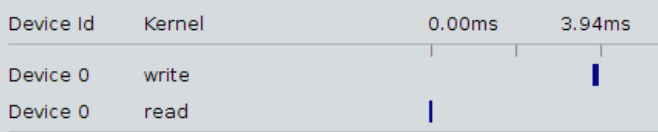
\includegraphics[width=0.7\textwidth]{Figures/profilerow}
\decoRule
\caption[profilerow]{ Dynamic Profiling result for row-stationary Implementation}
\label{fig:rowstatp}
\end{figure}

\begin{table}[]
\centering
\begin{tabular}{|l|c|c|}
\hline
\textbf{Implementation}        & \multicolumn{1}{l|}{\textbf{Execution Time (ms)}} & \multicolumn{1}{l|}{Frequency (MHz)} \\ \hline
\textit{Simple Implementation} & 0.15                                              & 256.1                                \\ \hline
\textit{Sliding Buffer}        & 0.09                                              & 252.8                                \\ \hline
\textit{Row Stationary}        & 3.94                                              & 184.4                                \\ \hline
\end{tabular}
\caption{Results of Part I Test}
\label{tab:resultpartone}
\end{table}

The profiling results and operating frequency of the board for each of the implementations is shown in table \ref{tab:resultpartone}. In the case of the row-stationary implementation, the compute array of processing elements are \emph{autorun} kernels. Therefore they are considered to be running the whole time during execution and will not be caught by the Intel Dynamic Profiler. To approximate the time consumed we take the time difference between the reader and writer kernels that communicate with the grid as the execution time.
Unsurprisingly, the row-stationary implementation is the slowest in a small example. One reason is a low operating frequency due to a long critical path of execution. Another reason is the synchronization and communication overhead between the processing elements in the processing grid. We see also that the sliding buffer has the best performance in the case of a single large image which also makes sense. In the next section we abandon the row-stationary implementation and test the two other kernels in a real-case scenario.


\subsection{Part II : Performance in a Real-Case} 

In \ref{testone} we used a very simple two dimensional convolution to benchmark three different convolution operators. Our row-stationary implementation doesn't support a real-case convolution with multiple input and output channels. For that we compare the two other implementations ( sliding buffer, and optimized implementation \ref{slidingimpl}) configured for a large batch of size of $ 2048 $ and for a convolution requiring multiple input and output channels. This allows us to better compare both operators and to choose which one is more suitable for the LeNet model. In fact, we use the third layer in LeNet as our benchmark \ref{tab:l3params}.

\begin{table}[]
\centering
\begin{tabular}{|l|l|}
\hline
\textbf{Parameter} & \textbf{Value} \\ \hline
Image              & 14x14          \\ \hline
Filter             & 5x5            \\ \hline
Input Channels     & 6             \\ \hline
Output Channels    & 15             \\ \hline
Batch Size         & 2048           \\ \hline
\end{tabular}
\caption{Configuration for Layer-3 LeNet}
\label{tab:l3params}
\end{table}

<add table with results>
<show area usage and compare area usage vs performance >
<show reports>
< and profile pipelining in both > 
<analysis is compare estimated latency vs. actual latency > 


%----------------------------------------------------------------------------------------
\section{Pipelined vs. Non-Pipelined Inference}

<waiting for compilation>


%----------------------------------------------------------------------------------------
\section{Training LeNet}

<needs some coding, then run it > 

%----------------------------------------------------------------------------------------
